% !TeX encoding = UTF-8
% !TeX program = pdflatex
% !TeX spellcheck = en_US

\documentclass[LaM,binding=0.6cm]{sapthesis}

\usepackage{microtype}

\usepackage{listings}
\lstset{
basicstyle=\small\ttfamily,
columns=flexible,
breaklines=true
}

\usepackage{hyperref}
\hypersetup{
			hyperfootnotes=true,			
			bookmarks=true,			
			colorlinks=true,
			linkcolor=red,
            linktoc=page,
			anchorcolor=black,
			citecolor=red,
			urlcolor=blue,
			pdftitle={Master Thesis - Deceptive Box: Whole-System Emulation Meets Evasive Malware},
			pdfauthor={Giulio Ginesi},
			pdfkeywords={thesis, sapienza, roma, university}
}

\usepackage[super]{nth}
\usepackage{color}
\usepackage{framed}

\newcounter{t0d0_counter}
\newcommand{\todo}[1]{
  \stepcounter{t0d0_counter}
  \definecolor{shadecolor}{rgb}{1,1,0} % this is yellow
  \begin{shaded}
  T0D0 \arabic{t0d0_counter}: #1
  \end{shaded}
}

% Commands for the titlepage
\title{Deceptive Box: Whole-System Emulation Meets Evasive Malware}
\author{Giulio Ginesi}
\IDnumber{1840066}
\course{Cybersecurity}
\courseorganizer{Facolt\`{a} di Ingegneria dell'Informazione, Informatica e Statistica}
\AcademicYear{2019/2020}
\copyyear{2020}
\advisor{Prof. Daniele Cono D'Elia}
% \advisor{Dr. Nome Cognome}
% \coadvisor{Dr. Nome Cognome}
\authoremail{ginesi.1840066@studenti.uniroma1.it}

% \examdate{16 April 2013}
% \examiner{Prof. Nome Cognome}
% \examiner{Prof. Nome Cognome}
% \examiner{Dr. Nome Cognome}
\versiondate{\today}



\begin{document}

\frontmatter

\maketitle

% \dedication{A (G)Anna}

% \begin{abstract}
% This document is an example which shows the main features of
% the \LaTeXe\ class \texttt{sapthesis.cls} developed by Francesco Biccari
% with the help of GuIT (Gruppo Utilizzatori Italiani di \TeX).
% \end{abstract}

\begin{acknowledgments}
Ho deciso di scrivere i ringraziamenti in italiano

\end{acknowledgments}

\tableofcontents

\mainmatter

% chapters, ideally one file per chapter
% !TEX root = ../main.tex
\chapter{Introduction}

Malicious Software (malware) has become increasingly common, and profitable, in the latest years. Usually, malware are differentiated based on their goal, some examples are: adware dedicated to displaying an advertisement on the user pc, spyware are the ones dedicated to monitoring the user, ransomware are the ones encrypting important files and asking for a ransom and so on. 

In the past, it was possible to clearly differentiate malware types based on their goal and their complexity. A modern example is Adware, these used to be really simple pieces of code, targeted to a broad group of people, hoping to generate the maximum profit. However, with the years even such pieces of malware started to become more sophisticated and to embed complex mechanisms to avoid detection, evade anti-virus software and even package more advanced features~\cite{bitdef}.

In order to detect such malicious pieces of code, it is important to understand how they work and interact with the system. The source code of a malware is rarely available for review therefore a different approach must be taken to understand the internal mechanisms of a program when only the final executable is available. 

For an executable to run on a system, it must be compiled. The compilation is the process of translating the source code of a program, written in a high-level language, into instructions that can be executed directly by the CPU. The process of understanding how a program works by reading and interpreting CPU instructions ``by hand'' is called Reverse Engineering.

Malware Analysis is the process of analyzing a malicious piece of code in order to extract as many information as possible from it. This is especially valuable to understand the capabilities of a malware but also to extract useful Indicator of Compromise (IoCs) that can be leveraged to detect an infection of a system. 

Malware analysis and detection is, therefore, a cat and mouse game in which the two parties engage in a never-ending chase trying to keep up with one another. For this reason, it is of paramount importance the analyst's arsenal is always up to date.

Malware Analysis is composed of many different phases and approaches depending on what is the final goal and the time available for the analyst. The two main phases are static analysis and dynamic analysis. Static analysis involves using different programs to extract information from the sample as well as reading through the assembly code. This is a very slow approach in which both the tools and the analyst can be easily fooled by the malware author in drawing the wrong conclusions. For this reason, dynamic analysis plays a major role in understanding the real capabilities of a binary. The main advantage is that, besides being faster than static analysis, IoCs can be collected in a semi-automated way by running the sample in carefully crafted environments. These are specialized virtual machines that allow the analyst to perform deep introspection of the running system.

\paragraph{The Problem with Evasive Malware.}
Malware authors do not want their programs to be analyzed and the more they are able to slow down the analysis the more are the chances that malware can spread and achieve its goal. For this reason, modern malware employs many different techniques to avoid detection and make the work of the analyst harder. When it comes to dynamic analysis, a particularly effective technique consists of fingerprinting the environment in order to detect the type of hardware and software present in the system. In this way, the malware can decide if the environment resembles a real one or not and hide its real capabilities accordingly, realizing a so-called \textit{evasion}.

As a matter of fact, virtual machines are the core of the dynamic analysis process as they allow to run the malware on controlled and isolated environments. Some of the most complex analysis systems are built on top of Virtual Machines based on Whole System Emulation frameworks which allow having fine-grained control not only over the code that is being run but also on the hardware. This has many benefits; for example, since the hardware is emulated, it is possible to carry out malware analysis of many different samples, even the ones designed for a different architecture, on top of an arbitrary system. Moreover, the ability to tap into different components and place custom pieces of code in very specific points of the emulation process, such as when the instructions are translated between one architecture and the other, allows to build very powerful and complex systems that are virtually invisible to the malware. Such capabilities are difficult to achieve in Virtual Machines solutions that build, instead, on hardware-assisted virtualization~\cite{Lastline2014FullSE}.

The most common Whole System Emulation system is QEMU, which is an open-source CPU and hardware emulator. This hardware abstraction step introduces some overhead but this is almost irrelevant compared to the great level of detail that can be achieved with this type of analysis. 

However, the fact that the system is virtualized inevitably introduces some artifacts in the environment. These can be of different types depending if they are introduced at hardware or software level. As a matter of fact hardware artifacts are present because the processors and other components are virtualized. On the other hand software artifacts are generated because some additional drivers are often required on the guest system for it to run properly. 

\paragraph{Contributions of the Thesis.}
The objective of this thesis is to enhance an existing analysis framework based on whole system emulation in order to make it completely transparent to the malware in the face of known evasion techniques. Specifically, we enhance PANDA~\cite{panda} (Platform for Architecture Neutral Dynamic Analysis) that has been used in several recent research works some examples are: Malrec~\cite{malrec} PANDAcap~\cite{pandacap} and Avatar$^2$~\cite{avatar2}. PANDA is based on QEMU and leverages a plugin system to perform many different analysis techniques. Our contribution consists of adding several anti-evasion plugins that make it possible to handle and run even evasive malware in such a framework, allowing existing plugins to perform a complete analysis. The newly created plugins are aimed at resolving 4 main problems: timing detection based on RDTSC, features detection based on CPUID, other mechanisms based on system call and API call. As evasion capabilities evolve over time the plugins must keep up with them. For this reason the plugins have been designed with extensibility in mind and to be as future proof as possible. As a matter of fact, new system calls or APIs can be added for any need without having to rewrite the plugin but simply using existing constructions. On the other hand, other plugins can be created based on the ones aimed at handling CPUID and RDTSC. This might be interesting for example to study how these two instructions behave in particular circumstances.


\medskip
\paragraph{Structure of the Thesis.} The remainder of the thesis follows this structure:

\medskip
In \hyperref[chap:2]{Chapter~\ref*{chap:2}:~\nameref{chap:2}} the most common techniques used to dissect malicious code are presented. This chapter will have a particular focus on evasive malware as they poses specific challenges in the dynamic analysis process. The most common evasive and fingerprinting techniques will be analyzed. The available environment testing suites will also be presented. 


\medskip
In \hyperref[chap:3]{Chapter~\ref*{chap:3}:~\nameref{chap:3}} the modern virtualization methods will be presented with a particular focus on QEMU and its whole system emulation capabilities. A short overview of the internal working mechanism of QEMU and its intermediate language TCG will be given. This translator and the QEMU structure are particularly important as they are at the base of the Panda framework and generally of dynamic analysis frameworks based on QEMU.


\medskip
In \hyperref[chap:4]{Chapter~\ref*{chap:4}:~\nameref{chap:4}} the panda-re analysis framework will be presented with particular focus on its plugin system and record/replay capabilities. Moreover a small comparison between this framework and other available ones will be given. 


\medskip
In \hyperref[chap:5]{Chapter~\ref*{chap:5}:~\nameref{chap:5}}  my contribution to the PANDA framework will be presented together with some of the challenges in extending its functionalities to cover the most common anti analysis techniques. In the end the results of running some anti-analysis test programs in the new version of the framework will be presented.

\medskip
In \hyperref[chap:6]{Chapter~\ref*{chap:6}:~\nameref{chap:6}} the conclusions and possible future works to further refine and enhance the framework are illustrated.
% !TEX root = ../main.tex

\chapter{Malware Analysis}
\label{chap:1}

\daniele{Add introductory text on the importance of having efficient and semantically rich techniques for analyzing malware, the different trade-offs for different levels of inspection, and the heterogeneous alternatives available}

\section{Static and Dynamic Approaches}
There are two types of analysis techniques that can be used to fully understand and dissect a malicious piece of code.

\subsection*{Static Analysis (and Its Challenges)}

\textit{Static analysis} is the process of analyzing a, possibly, malicious piece of software without running it on the machine. This is usually done with the aid of different tools to parse the header of the executable and to extract as many information as possible. Subsequently the malware can be analyzed using a disassembler which is a program that allows the user to take the machine code and "reassemble" it to a higher level, human readable, code. Such process can be taken even further with the use of a decompiler, this software tries to bring a higher level of abstraction into the reversing process by decompiling machine code into a pseudo-language often similar to C reducing the effort required by the analyst to interpret machine code.

This kind of analysis is usually very time consuming and requires deep understanding of the underlying architecture of the processor. Moreover the malware author can use different techniques to modify the compiled code making it harder to reverse engineer or even to trick the analyst into believing that the code has different capabilities than the real ones. These techniques are commonly referred as \textbf{Obfuscation} however there are many different techniques that are used to hide malware capabilities: \textit{Encryption, Packing, Obfuscation, Polymorphism, Metamorphism}.\cite{Ye2017ASO}

\textit{Encryption} and \textit{Obfuscation} are similar techniques used to hide pieces of the malicious code not only from the analyst but also from antivirus software. At low level often \textit{Encryption} consists of performing a \textit{XOR} operation on a defined portion of memory while \textit{Obfuscation} involves masquerading API calls and split strings in the code in order to make it harder to understand the real behaviour of the malware.

On the other hand \textit{Packing} consists in encrypting and compressing the real code of the malware and, instead of shipping the "real" malicious code, the packed version will feature an unpacking stub which will take care of extracting and then running the malware directly into the memory making it harder to detect and reverse engineer.

Finally \textit{Polymorphism} and \textit{Metamorphism} are conceptually similar, the first one involves a polymorpic engine which allows to compile the code in a non deterministic way meaning that it will be different at each compilation but it will however still retain all the initial functionalities, this is usually achieved also with the use of encryption. \textit{Metamorphism} on the other hand is a really interesting technique through which the code of a program can be modified at run time adding a great layer of complexity and opening the door to a dedicated category of malware.

The Static Analysis is a powerful technique however for some more advanced pieces of malware it is not enough and instead it is required to run the malicious code in order to fully understand the capabilities and interactions with the machine.

\subsection*{Dynamic Analysis}

\daniele{Too dry: your thesis is around dynamic analysis! Detail the different execution technologies available to date, and emphasize why whole-system emulation is important for fine-grained analysis of malware and in general for software security topics (e.g. for whole-system information flow tracking, you can cite the DECAF papers}

\textit{Dynamic analysis} is the process of running the malicious program in a controlled environment, this is usually a virtual machine with proper measures in place to avoid external communication and instead capture and analyze network traffic. Such virtual machines are also equipped with introspection tools such as \textit{process monitor, process explorer, fakenet-ng} and similar allowing the malware analyst to deeply investigate the behaviour of a malicious program.

This kind of analysis involves running the sample with a debugger attached, a debugger allows the analyst to inspect the internal structure of the machine at runtime having direct access to CPU registers, process memory and allowing the user to modify the control flow of a program using breakpoints, inserting custom instructions and modify the memory during execution. 

There are also ad-hoc sandboxes used to automatically run a malware and then collect all the different interactions with the system producing then a detailed report. This is often referred as automatic malware analysis and the most common sandboxes are cuckoo\footnote{\url{https://cuckoosandbox.org/}}, joe sandbox \footnote{\url{https://www.joesandbox.com/}} and VMRay \footnote{\url{https://www.vmray.com/}}. 

In most cases the best analysis technique is a combination of the two. As a matter of fact debuggers are often used to unpack malware by setting breakpoints in the code and running it in a controlled environment until the real malware is extracted and loaded into memory, the resulting piece of code can then be dumped to disk and statically analyzed. 

\section{Evasive Malware}
\label{sec:evmal}

As mentioned previously the Dynamic Analysis takes place inside a controlled environment. Having a real computer, isolated from the network and re-imaged every time that a sample is analyzed is the best scenario but also highly inefficient. There are different technologies, such as Virtual Machines, that are used nowadays to achieve the same results but with less effort, overhead and a great saving in terms of costs. 

From an attacker prospective detecting if the current machine is a physical one or a virtual one can really make the difference as the more it takes for an analyst to reverse a sample the more it can stay in the wild and perform malicious actions. In addition to this, testing for the presence of a debugger installed in the system or attached to the program is another form of protection that is used by the malware to avoid the analysis process.

There are multiple techniques used to detect if a piece of code is running in an analysis environment. According to \cite{9018111} such techniques can be divided in two categories:
\daniele{Inaccurate: red pills originally detected emulators, but you should say that now you can use them to detect anomalies when executing instructions or looking up the position of specific structures in memory (see VMware artifacts) on a hypervisor or any other dynamic execution platform that is not a bare-metal machine}

\begin{enumerate}
    \item \textbf{Red Pills} used to detect if a CPU is emulated. As detailed in \cite{bruschi} these usually consists of different sets of opcodes that behaves differently depending if they are executed inside a physical or virtualized environment. However in addition to classical red pills emulators can also be detected by leveraging hypervisor calls such as CPUID and other particular instructions such as RDTSC.
    \item \textbf{Virtualization Artifacts} are peculiar characteristics of a machine that are introduced with virtualization. Most notably virtual machines, due to their nature, leave some distinctive fingerprints in the system.
\end{enumerate}

The CPUID instruction\footnote{\url{https://c9x.me/x86/html/file_module_x86_id_45.html}} (shorthand for CPU IDentification) is one of the most used and interesting \textbf{Red Pills} as it can produce a good amount of details about the processor and the environment in general.

CPUID reads the input parameter from the \textit{EAX} registry and places the outputs in the \textit{EAX, EBX, ECX, EDX} registries. The length of the result is variable and therefore different registers are used according to the initial \textit{EAX} value. From a virtualization detection prospective the most interesting results are obtained by calling this instruction with the \textbf{0x1}, \textbf{0x40000000} and \textbf{0x80000000}\cite{CPUID}. 

When calling \textit{CPUID} with 0x1 as parameter the CPU feature information are returned in \textit{ECX} and \textit{EDX}. The last 3 bits of the value in \textit{ECX} are reserved and the \nth{2} of those (i.e. the \nth{31}) bit is called Hypervisor bit, physical CPUs sets this bit to 0 while virtual ones set this bit to 1. This is a simple and fast way to detect if a program is running under a virtualized environment. 

In addition to this calling \textit{CPUID} with 0x40000000 as parameter will return the Hypervisor Brand information in \textit{EAX, ECX, EDX}. While calling \textit{CPUID 0x80000000} will return the CPU Brand information in the \textit{EAX, EBX, ECX, EDX} registries. Obviously both of the above information are set to specific values if the environment is virtualized. 

Another interesting instruction is \textit{RDTSC} \footnote{\url{https://c9x.me/x86/html/file_module_x86_id_278.html}} this is used to read the processor timestamp counter, which is a 64 bit values that stores the number of cpu cycles elapsed since the last reset. Lower bits are stored in the \textit{EDX} register while higher bits are stored in the \textit{EAX} register. The difference between two subsequent executions of this instruction on a physical CPU will be low while it will be a much higher number on virtual CPUs.

On the other hand \textbf{Execution Artifacts} are very dependant on the virtualization system used and can be found in different places of the system. One of the most obvious artifact is the MAC Address of the network interfaces which, by default, is set to well known values by all the different Virtualization Software as in Figure \ref{fig:vms}.

\noindent
\begin{figure}[htp]
\centering
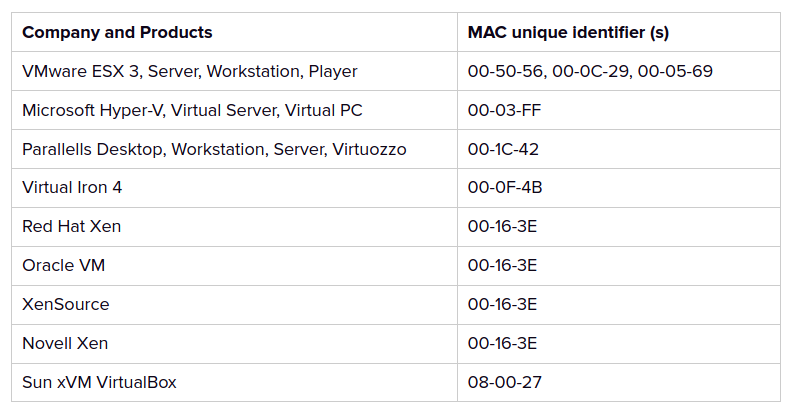
\includegraphics[width=\linewidth]{images/vms-mac-address.png}
\caption{Common VMs mac addresses \newline \url{https://www.techrepublic.com/blog/data-center/mac-address-scorecard-for-common-virtual-machine-platforms/}}
\label{fig:vms}
\end{figure}

Another common source of information for evasive malware is the windows registry, this is defined in the official documentation as a central hierarchical database used to store information that is necessary to configure the system for one or more users, applications, and hardware devices.

\textit{"The Registry contains information that Windows continually references during operation, such as profiles for each user, the applications installed on the computer and the types of documents that each can create, property sheet settings for folders and application icons, what hardware exists on the system, and the ports that are being used."}\cite{windocs}

The windows registry has a well defined structure, it is organized as a tree and each node in the tree is called a \textit{key}. Each \textit{key} in the registry can contain both \textit{sub-keys} and data entries called \textit{values}. Each \textit{key} has at least 1 value called \textit{Default}. The name of each \textit{key} consists of one or more characters and is case insensitive. Sometimes the presence of a \textit{key} it is sufficient for the application to store a certain setting, other times a \textit{key} will have different \textit{values} representing a piece of information. \textit{Values} can have many different types according to the information they are holding, the most common values are \lstinline{REG_BINARY, REG_DWORD} and \lstinline{REG_SZ}. 


An example of virtualization artifact related to the registry is the \textit{SystemBiosVersion} value which for VirtualBox and QEMU is as follows:
\begin{itemize}
    \item \lstinline{HARDWARE\Description\System (SystemBiosVersion) (VBOX)}
    \item \lstinline{HARDWARE\Description\System (SystemBiosVersion) (QEMU)} 
\end{itemize}

Other virtualization artifacts are system files and drivers such as, among the others:
\begin{itemize}
    \item \lstinline{system32\drivers\vmci.sys}
    \item \lstinline{system32\drivers\VBoxVideo.sys}
    \item \lstinline{system32\vboxtray.exe}
\end{itemize}

Moreover other structures like ACPI tables, SMBIOS strings as well as Disk Size and RAM Size can be used to fingerprint the system and reveal the presence of a virtual machine. 


\section{QEMU and Emulation Artifacts}
\daniele{give some context on QEMU, explain why relevant (you will say it in the introduction, but every chapter should be self-contained so to  speak), how dynamic binary translation behind it works, and expand the information you already have below}

QEMU due to its nature is one of the virtualization systems with the lowest footprint on the guest. Taken directly from the Al-Khaser github repository\footnote{\url{https://github.com/LordNoteworthy/al-khaser}} the artifacts used to fingerprint QEMU are the following:

\begin{itemize}
    \item \lstinline{HARDWARE\DEVICEMAP\Scsi\Scsi Port 0\Scsi Bus 0\Target Id 0\Logical Unit Id 0 (Identifier) (QEMU)}
    \item \lstinline{HARDWARE\Description\System (SystemBiosVersion) (QEMU)}
    \item \lstinline{SetupAPI SetupDiEnumDeviceInfo (GUID_DEVCLASS_DISKDRIVE)}
    \item \lstinline{SMBIOS string checks (Qemu)}
    \item \lstinline{ACPI string checks (Qemu)}
    \item \lstinline{qemu-ga.exe (QEMU)}
\end{itemize}

as well as the above mentioned \textit{CPUID} which will return specific strings both for QEMU alone or if used in combination with KVM.


\section{Environment Testing Suites}

\daniele{Explain why they are important, how they summarize what we learn from malware in the wild (so people can't tell you that you techniques are unlikely to be effective on the average sample in the wild), and mention other sources: VMDE, SEMS, the CheckPoint collections for VM detections and anti-debug tricks, elaborate on how some techniques are general and affect multiple execution technologies (e.g. slowdown measurements vs dynamic analysis)}

There are available online different tools to perform automatic checks of the environment which aims to stress test the machine and verify how hidden is the analysis environment. The two most famous ones are Al-Khaser and Paranoid Fish\footnote{\url{https://github.com/a0rtega/pafish}}. Those tools are based on real techniques employed by malware to detect sandboxes and analysis environment and will run all the tests in sequence producing a final report of the passed and failed tests.

Paranoid Fish is a slightly older project which appears not to be maintained anymore while Al-Khaser is the evolution of Paranoid Fish and features many more techniques. It is important to note that not all the implemented techniques are a reliable indicator of the presence of a Virtual environment. Some checks such as the disk size, number of cores or the ram size might still fail even on computers still in use today. 

\todo{Add screenshots of the frameworks} 

\section{Remarks}
\daniele{Now you should be paving the way on what you will describe in your thesis. In this chapter or in the next one you should draw also some comparison with hypervisor-based monitoring and instrumentation (DRAKVUF, Ether, etc) and explain that they do not help for some tasks that require whole-system emulation instead, or their instrumentation facilities are not flexible enough to allow some detailed analyses. If you do it in the next chapter, here you should be saying a few anticipatory things too.}
\chapter{Whole System Emulation}

\section{Virtual Machines}

\subsection{qemu}

\section{Other possible approaches}

\chapter{panda-re}

\textbf{Panda-re} or just \textbf{PANDA} (\textbf{P}latform  for  \textbf{A}rchitecture-\textbf{N}eutral  \textbf{D}ynamic  \textbf{A}nalysis) is a framework based on QEMU which provides a programmatic interface to perform deep virtual machine and operating system introspection. It has been designed to be a platform to perform reverse engineering of complex pieces of malware thanks to its ability to record and replay executions. However the functionality is obviously not limited to malware analysis but this framework can be used in all those cases requiring a deep understanding of how a software works or a specific type of analysis such as taint analysis. The typical workflow when using \textbf{PANDA} can be seen in Figure \ref{fig:wkflow}.

\begin{figure}[htp]
\centering
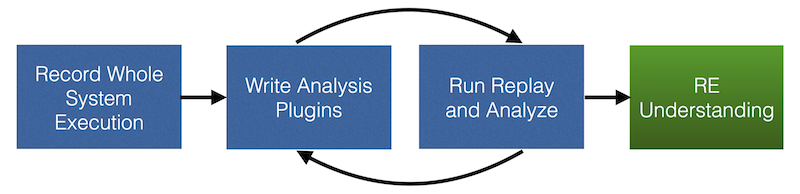
\includegraphics[width=\linewidth]{images/panda_workflow.png}
\caption{Typical panda workflow as desciribed in the documentation.}
\label{fig:wkflow}
\end{figure}


\section{Framework overview}

\textbf{PANDA} leverages the full system emulation capabilities of QEMU, this supports 13 types of CPU architectures while \textbf{PANDA} has built in support for 3 of them: x86, powerPC and ARM. 

Building on top of QEMU architecture \textbf{PANDA} exposes an interface to control the Virtual Machine internal state as well as to access all code and data on the guest operating system. In this way different techniques such as Taint Analysis or Operating System Introspection can be applied.

One of the main components of the framework are \textbf{callbacks}, these are essentially functions that are called when specific events happens inside the virtual machine. Each \textbf{callbacks} is usually called before and after the define event takes place, the relevant function can be selected by using the \textit{before} or \textit{after} prefix (e.g. \lstinline{before_block_exec} and \lstinline{after_block_exec}).

An exhaustive list of available \textbf{callbacks} can be found in the documentation\footnote{\url{https://github.com/panda-re/panda/blob/master/panda/docs/manual.md#appendix-a-callback-list}} however they can be conceptually divided into 4 main categories:

\begin{itemize}
    \item \textbf{Execution Callbacks} are generic callbacks used to trace execution of code inside the virtual machine. There are different levels of granularity that this callbacks provide reflecting events inside the virtual machine, usually at CPU level. Example of this events are: asid change, block execution, block translation or single instruction.
    \item \textbf{Memory Callbacks}, which must be enabled on demand, are called when there is an interaction with the virtual or physical memory. 
    \item \textbf{Replay Only Callbacks} are executed only during replays and usually utilized to handle things like DMA, network interaction and similar.
    \item \textbf{Management Callbacks} are used to perform actions when specific actions related to QEMU takes place, for example when the monitor interface is used.
\end{itemize}

A visual representation of the emulation stage at which the various callbacks are executed can be seen in Figure \ref{fig:calls}.

\begin{figure}[htp]
\centering
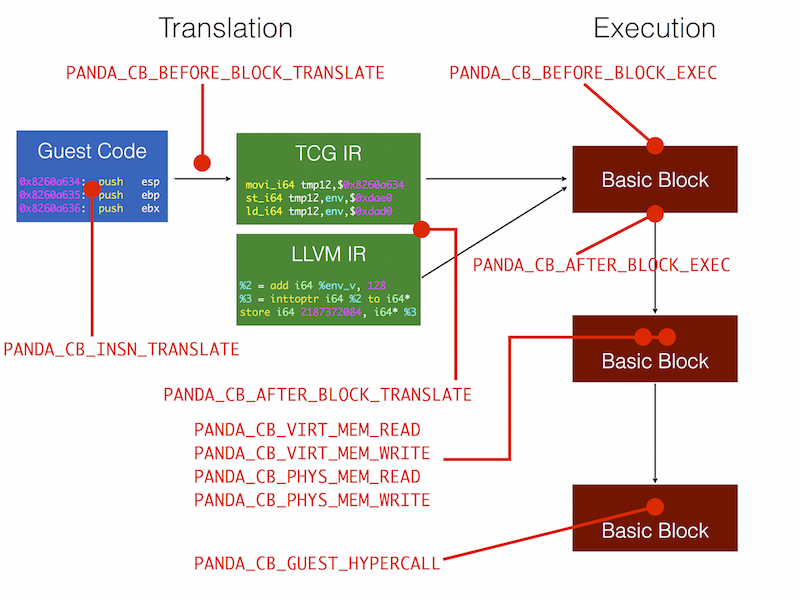
\includegraphics[width=\linewidth]{images/callback_diagram.png}
\caption{Main callbacks and different triggering points. }
\label{fig:calls}
\end{figure}

In addition to callbacks there are some helper functions that are exposed by \textbf{PANDA} in order to make the interaction with QEMU easier. The CPU internal state is saved in a structure called \lstinline{CPUState}, at each time of the execution this structure is made available through a global pointer called \lstinline{env}. 

Moreover \textbf{PANDA} exposes two functions to interact with the Virtual Machine memory: 
\begin{enumerate}
    \item \lstinline{int panda_physical_memory_rw(target_phys_addr_t addr, uint8_t *buf, int len, int is_write);} allowing to read or write bytes, according to the \lstinline{is_write} parameter, at \lstinline{addr} in the pysical memory.
    \item \lstinline{int panda_virtual_memory_rw(CPUState *env, target_ulong addr, uint8_t *buf, int len, int is_write);} which is the same as the above function but used to operate on virtual addresses.
\end{enumerate}


In addition to the above \textbf{PANDA} itself provides some default plugins to perform many different tasks and that can be used as the foundation to further expand analysis capabilities.


\subsection{Plugin system}

The plugin system is the heart of PANDA, a plugin is a piece of code which extends panda functionalities in order to perform specific actions on the running system. Usually a plugin observe the what is happening in the system and either exposes some \textbf{callbacks} that can be used by other plugins or prints information to the user.

\textbf{Callbacks} exposed by a plugin in order to be used by another are called plugin to plugin interface (or \textbf{PPP}) such system allows for the creation of low level plugins that are responsible only to add more functionalities into the \textbf{PANDA} environment, example of such plugins are hooks, syscalls2 or OSI. These are useless if not used in combination with a custom code that takes care of using the \textbf{PPP} exposed by each of them to perform specific actions at well defined execution points.

As it can be easily understood plugins can also be used in combination with helper function to alter the Virtual Machine internal state at run time. As a matter of fact every single component of the VM can be accessed both in read and write mode and this gives the ability to the user to precisely control the execution flow or to introduce custom code or data inside the system whith minimal interaction with it. 


\subsubsection{Plugin writing}

Plugins can be written in C or C++, in order for them to be compiled and enable into PANDA a specific folder structure is required. Such structure is outlined in \ref{fig:plugs}

\begin{figure}[htp]
\centering
\begin{minipage}{\linewidth}
\dirtree{%
.1 panda.
.2 panda.
.3 plugins.
.4 my plugin.
.5 Makefile.
.5 README.md.
.5 myplugin.c.
.4 config.panda.
}
\end{minipage}
\caption{Plugins folder structure}
\label{fig:plugs}
\end{figure}

The Makefile is most of the time standard and provided by PANDA, it can be seen in Figure \ref{fig:mak}

\begin{figure}[htp]
\centering
\begin{minipage}{\linewidth}
\begin{lstlisting}
# Don't forget to add your plugin to config.panda!

# If you need custom CFLAGS or LIBS, set them up here
# CFLAGS+=
# LIBS+=

# The main rule for your plugin. List all object-file dependencies.
$(PLUGIN_TARGET_DIR)/panda_$(PLUGIN_NAME).so: \
	$(PLUGIN_OBJ_DIR)/$(PLUGIN_NAME).o
\end{lstlisting}
\end{minipage}
\caption{Basic Makefile}
\label{fig:mak}
\end{figure}

Moreover each plugin should expose at least the following two functions: \lstinline{bool init_plugin(void *)} \lstinline{void uninit_plugin(void *)}.

The first one is called during plugin initialisation and is where the different functions and callbacks are initialized. The second one is called when panda is terminating or when the plugin is unloaded and is typically used to clean up custom structures initialized by the plugin.

In addition to this the plugin should import the following file \lstinline{#include "panda/plugin.h"} which is essentially the \textbf{PANDA} API. Lastly the name of the plugin should be added to the \lstinline{config.panda} file in order for it to be automatically compiled during panda compilation.


\subsection{Record and Replay}

In addition to the above plugin system \textbf{PANDA} also features a method to record the entire state of the machine and replay that later in a deterministic way. This leverages the \textbf{rr} (record and replay) framework from Mozilla which was usually developed to extend gdb functionalities and allow for time travel debugging. 

\textit{"You record a failure once, then debug the recording, deterministically, as many times as you want. The same execution is replayed every time."}\footnote{\url{https://rr-project.org/}}

This enables writing complex and articulated plugins and allows for faster analysis, as a matter of fact plugins introduce overhead in the execution. Recording the execution of a malware without any plugins enabled and then run them on the recording allows to get rid of a lot of that overhead. This is the typical workflow as in Figure \ref{fig:wkflow}. Due to the fact that the replay is deterministic it will have the same result at every run. It means that the results are the same as if the machine is booted up, the OS is started and initialized, possibly some modifications applied and then run the program to be analyzed. This has however some limitations as explained on the\textbf{rr} website: 

\textit{"Unlike many record and replay implementations, we do not record the inputs to devices; this means that one cannot "go live" during a recording, but it greatly simplifies the implementation. To get an idea of what is recorded, imagine drawing a line around the CPU and RAM; things going from the outside world to the CPU and RAM, crossing this line, must be recorded."}

A recording can be taken via the QEMU monitor interface using the \lstinline{begin_record <replay name>} and \lstinline{end_record} commands, this will create two files: \lstinline{<replay name>-rr-snp} which is a snapshot of the VM at the beginning of the recording and \lstinline{<replay name>-rr-nondet.log} which will hold a log of all non deterministic inputs during the recording. A recording can then be replayed by adding the \lstinline{-replay <replay name>} command line argument to the panda executable. 

Plugins are generally used for analysis therefore they rarely modify directly the virtual machine environment but instead they focus on catching particular behaviours and logging it or perform some more analysis based on specific events happening inside the virtual machine. As mentioned before in order for the replay functionality to be used it is important that the plugin doesn't alter the control flow of the program, as a matter of fact due to the nature of \textit{rr} (\underline{deterministic} record and replay) if a replayed trace diverges from what has been recorder (for example the program takes a different conditional jump) it will no longer be able to continue the replay as it will not be able to find what should be replayed anymore. For this reason plugins that introduce modifications in the virtual machine, such as hiding specific virtualization artifacts, must be run on the live system. In the same way it is not possible to perform analysis that will make the execution diverge from the recording, this means for example that during the analysis of a malware the Command and Control communications must be deterministic and is not possible to record just 1 interaction with the C2 and then bruteforce all the possible commands during the replay.


\subsection{Python bindings}

In addition to the above mentioned plugins system \textbf{PANDA} exposes also a Python interface, this is referred to as \textbf{pypanda}. The documentation for the python package can be found at \url{https://panda-re.github.io/panda.html}. Such interface allows for better scriptability and to have faster prototyping. Everything that can be done with a "standard" C/C++ plugin can be accomplished with Python moreover, \textbf{pypanda} exposes some high level functions that can be used to write entire scripts to automatically run a self contained simulation.

In addition to this there are some C/C++ plugins created to be used specifically with \textbf{pypanda}, for example the hooks plugin, as mentioned in issue 613\footnote{\url{https://github.com/panda-re/panda/issues/613}}:

\textit{"It's designed to be used with the python interface which has some code to ensure the hook only runs when in the right process so you'd either need to reimplement that logic or use the python interface"}

While proper plugins are somehow specialized pieces of code designed to analyze or act on a specific behaviour python code can interact directly with \textbf{PANDA} and can be used not only to build new plugins but also to control the entire simulation life cycle without the user having to interact with the command line or on the qemu monitor.

\textbf{pypanda} exposes a class used to interact with \textbf{PANDA}: \lstinline{class Panda (arch='i386', mem='3G', expect_prompt=None, os_version=None, qcow=None, os='windows', generic=None, raw_monitor=False, extra_args=[])}, this accepts different parameters to create a well defined virtual machine. The newly created VM can then be used to run either a live system or a recording, obviously if run on the recording this should have been taken on a VM with the same system configuration. 

There is a small overhead when utilizing \textbf{pypanda} due to the nature and efficiency of the python code which is naturally different from pure C/C++ implementations however, as mentioned before, there are some operations such as setting hooks that are designed to be done mainly via the python interface. Moreover the python library exposes some more convenient methods to access internal structures compared with classical \textbf{PANDA} APIs. 

From the python interface it is possible to access not only \textbf{PPP} interfaces but also classical python callback, this as mentioned before allows for very complex interactions to be written in python. As a matter of fact there are different helper functions such as \lstinline{get_mappings, get_process_name, ...} that provides direct interfaces to other plugins such as OSI, hooks, taint and others. The function \lstinline{run} or \lstinline{run_replay} can then be used to run the simulation. Other helper functions include \lstinline{record} and \lstinline{end_record} used to control the recording, this allows to write python scripts that automatically run a simulation on the live system, records it, then runs some specific plugins on the recording. 

\section{Advantages compared to its competitors}
\todo{A lot of features, nice interface, record and replay}
There are other similar projects such as TEMU, DECAF and DRAKWUF however PANDA has some advantages and useful functionalities that can be helpful for analyzing evasive malware and to implement a sthealt VM.

One of the most interesting features of PANDA is the ability to record and replay execution. In particular in relation to evasive malware this is useful as it is possible to write a plugin to hide virtualization artifacts from the system and then run a malware on such system recording its execution. Others plugins can then be used on the replay to perform a proper malware analysis. 

Moreover exposing a python interface, although this introduces a bit of overhead, is a great feature compared to the other frameworks which allows for great scriptablility of actions and fast prototyping of complex experiments.
\chapter{Deceptive Box: PANDA meets evasive malware}
\label{chap:5}

As discussed before some particular categories of malware have been developed with specific checks in order to finely fingerprint the environment they are in to check for any sign of virtualization. This means that in order for them to be analyzed some specific virtual machines in which artfacts have been carefully removed and masqueraded are needed.

The goal of this thesis was to develop a set of Panda plugins that can be used to modify the Virtual Machine and Operating System internal state, at run time, in order to hide virtualization artifacts from the system. In this way Evasive Malwares can be run on a Fully Emulated System invalidating their attempts to fingerpint the environment and therefore having them to reveal their real capabilities.
By using Panda for this there are tree advantages: 
\begin{enumerate}
    \item The system can be monitored and modified at run time in order to counter any evasion attempt. 
    \item Due to the fact that it works in full system emulation mode it provides an external view of the system which is segregated but inspectable.
    \item The ability to record and replay allows for a malware to be run once on the live system and then analyzed later.
\end{enumerate}

In the following sections the 4 main contributions will be presented: 

\section{Leveraging panda-re to manipulate the live system}

As widely discussed in the previous chapters \textbf{PANDA} provides many useful features that can be used to modify a running virtual machine. Blindly faking results for different functions or instructions in a system is dangerous as most of them will likely be used by many other programs and giving wrong or arbitrary information might lead to system instability and crashes. Therefore all the plugins written needs to be aware of the target process that needs to be patched.

Instead of hiding every single artifacts left by QEMU on the system the preferred way was to analyze what ParanoidFish and Al-Khaser could find and focus on patching those, subsequently, the plugin can be extended to support different evasion techniques. Due to the nature of this project the resulting plugins will need to be run both on live and replay modes. As a matter of fact the plugins will introduce deep modifications in the system that, due to the way in which the record/replay system works, will need to be run always in order to maintain the integrity of the system during replays.

Some of the hardware based checks can be avoided simply by fine tuning the system, in particular the disk size and RAM size can be adjusted to avoid the detection by setting the RAM to a value greater that 1 GB and the disk to a size greater than 60GB. 

Some of the plugins used to patch the system are designed to be used with the python interface of \textbf{PANDA}, in particular the hooks plugin. Using the python interface will introduce a big overhead in the virtual machine therefore in order to try to reduce it at minimum only it was used only when really necessary (i.e. to perform api hooking). In addition to this it was necessary to create a new \textbf{PANDA} callback in order to have control of the Time Stamp Counter (TSC) during emulation.  

The \textbf{PANDA} plugins directly used for this project are: 

\begin{itemize}
    \item \textbf{osi} or Operating System Introspection was used to interface with the guest Operating System in order to extract for example the list of running programs or the list of loaded libraries. The peculiarity of this plugin is that it puts a layer of abstraction on top of the Operating System making it easy to write a plugin that will then work on all the supported OS.
    
    \item \textbf{syscalls2} is a plugin that provides a Plugin to Plugin interface each time a system call is executed. This plugin uses osi under the hood to perform system calls hooking, this allows for a breakpoint to be placed either when the syscall is executed or when the execution returns from the above sytem call. This latter part is particularly useful when exploring or changing the information returned from a specific syscall.
    
    \item \textbf{hooks} is a plugin that allows the user to specify a address and a function, the function will then be called each time that specific address is reached. This is essentially what a breakpoint is in a debugger.
    
    \item \textbf{hooks2} is the replacement for the hooks plugin however it is not yet completed and not all functionalities are working correctly however it provides some useful PPP interfaces. In particular \lstinline{on_process_start} and \lstinline{on_process_end} were used to execute specific actions when the monitored program was started.
\end{itemize}

Newer versions of windows are not supported by many of these plugins therefore in order to perform the analysis it was decided to use the most recent supported version which is Windows 7 32 bit.
Moreover as cited before, in order for the \textbf{PANDA} plugins to work, it is necessary to use QEMU without the KVM acceleration, this greatly lowers the performance of the system as the instrumentation system introduces a high overhead in the emulation and translation phase. 

\subsection{System call hooking}

The first approach was to write a \textbf{PANDA} plugin to hook system calls associated with typical footprinting performed by evasive malware. This involves having a deep understanding of how the Operating System works and which are its internal structures. A common source of information is the windows registry, there are 3 system calls that are used to access the registry: \lstinline{NtQueryValueKey, NtOpenKey} and \lstinline{NtEnumerateKey}. 

Using the \textbf{syscalls2} plugin different breakpoints were placed on the above mentioned system calls, in particular it was decided to capture the data returned by the above mentioned system calls. As \textbf{PANDA} is based on QEMU/BOCHS these are two of the strings that will be searched in different registry values. \lstinline{NtEnumerateKey} and \lstinline{NtOpenKey} are useful to catch enumeration however, \lstinline{NtQueryValueKey} is the syscall that provides the final string used for detection.

\lstinline{NtQueryValueKey} is the user mode version of \lstinline{ZwQueryValueKey}. This function allows to query the content of a value inside a specific registry key. In particular the key to be queried must have been accessed before with the \lstinline{NtCreateKey} or \lstinline{ZwOpenKey}, these functions will return a \textit{KeyHandle} that identify that specific key and that must be passed as parameter to the \lstinline{NtQueryValueKey} function. In addition to this there are some other values required to properly query the registry key, in particular \textit{ValueName} holds the name of the value to be queried. \textit{KeyValueInformationClass} specify the type of information to be returned and Length specify the length of the output buffer called \textit{KeyValueInformation}. The complete header of such function can be seen in Figure \ref{fig:querykey}.

\begin{figure}[htp]
\centering
\begin{lstlisting}[language=C]
NtQueryValueKey(
  IN HANDLE               KeyHandle,
  IN PUNICODE_STRING      ValueName,
  IN KEY_VALUE_INFORMATION_CLASS KeyValueInformationClass,
  OUT PVOID               KeyValueInformation,
  IN ULONG                Length,
  OUT PULONG              ResultLength );
\end{lstlisting}
\caption{\lstinline{NtQueryValueKey} header}
\label{fig:querykey}
\end{figure}

The \textit{KeyValueInformationClass} is particularly interesting as based on this value the type of information returned inside the \textit{KeyValueInformation} changes.

A common enumeration technique to detect QEMU consists of querying the value \textit{SystemBiosVersion} which is found under the path \lstinline{HKEY_LOCAL_MACHINE\HARDWARE\Description\System} and comparing it with the string \textit{BOCHS}.

In order to patch the above described System Call using \textbf{PANDA} it was necessary to hook the function when it returns, this can be done in the C plugin by registering to use appropriate \textbf{PPP} callback in the \lstinline{init_plugin} section. The implementation can be seen in Figure \ref{fig:pinit}.

\begin{figure}[htp]
\centering
\begin{lstlisting}[language=C]
bool init_plugin(void *self) {
    panda_require("syscalls2");
    [...]
    PPP_REG_CB("syscalls2", on_NtQueryValueKey_return, NtQueryValueKey_return);
    [...]
    return true;
}
\end{lstlisting}
\caption{Snippet of code representing how to hook the \lstinline{NtQueryValueKey} function.}
\label{fig:pinit}
\end{figure} 

The above snippet of code will run the \lstinline{NtQueryValueKey_return} function every time the \lstinline{NtQueryValueKey} returns, it is therefore necessary to have specific checks in place in order to patch the system only when the system call is executed from within a specified program. This has been implemented with a check on the program name or on the PID. Details of the patching function can be seen in Figure \ref{fig:pfun}. The function, after checking if the program running is the one specified for analysis, checks if the queried value is \textit{SystemBiosVersion} then if the value corresponds to \textit{BOCHS} it will replace it with \textit{INTEL}. It is important to note that all the particular structures used by this functions had to be ported from the windows library to this plugin in order for them to be used. Moreover the \lstinline{guest_wstrncpy} function is a helper function used to copy strings from the memory as it can be seen in \ref{fig:gstrin}.

\begin{figure}[htp]
\centering
\begin{lstlisting}[language=C]
void NtQueryValueKey_return(
    CPUState* cpu,
    target_ulong pc,
    uint32_t KeyHandle,
    uint32_t ValueName, 
    uint32_t KeyValueInformationClass,
    uint32_t KeyValueInformation,
    uint32_t Length, 
    uint32_t ResultLength 
    ){ 
    if (check_pid(cpu, tpid, tname)){
        char *name;
        UNICODE_STRING vname;
        name = malloc(1024*sizeof(char));
        panda_virtual_memory_rw(cpu, ValueName, (uint8_t *)&vname, sizeof(UNICODE_STRING), 0); // extract the pointer to string
        guest_wstrncpy(cpu, name, 1024, vname.Buffer); // read the string
        if (strcmp(name, "SystemBiosVersion")==0){
            KEY_VALUE_PARTIAL_INFORMATION rr;
            panda_virtual_memory_rw(cpu, KeyValueInformation, (uint8_t *)&rr, Length, 0);
            if (rr.Data[0]=='B' && rr.Data[8] == 'S'){
                // printf("\n\tPatching BOCHS\n");
                for(int i=0;i<5;i++){
                    char sub[6] = "INTEL";
                    rr.Data[(i*2)] = sub[i];
                }
                panda_virtual_memory_rw(cpu, KeyValueInformation, (uint8_t *)&rr, Length, 1);    
            }
        }
        free(name);
        return;
    }
}
\end{lstlisting}
\caption{Patching the value inside the registry using the \lstinline{NtQueryValueKey_return} function.}
\label{fig:pfun}
\end{figure} 

\begin{figure}[htp]
\centering
\begin{lstlisting}[language=C] 
uint32_t guest_wstrncpy(CPUState *cpu, char *buf, size_t maxlen, target_ulong guest_addr) {
    buf[0] = 0;
    unsigned i;
    for (i=0; i<maxlen; i++) {
        panda_virtual_memory_rw(cpu, guest_addr + 2 * i, (uint8_t *)&buf[i], 1, 0);
        if (buf[i] == 0) {
            break;
        }
    }
    buf[maxlen-1] = 0;
    return i;
}
\end{lstlisting}
\caption{\lstinline{guest_wstrncpy} function implementation.}
\label{fig:gstrin}
\end{figure}

This is an effective method to patch various system calls and can easily be expanded for any other syscall used for Virtualization detection.


\subsection{CPUID hooking}

A robust detection technique employed by malware involve taking advantage of the information provided by the \lstinline{CPUID} instruction as detailed in Section \ref{sec:evmal}. In order to patch the values returned by this instruction it is possible to use a callback already available in \textbf{PANDA}: \lstinline{PANDA_CB_GUEST_HYPERCALL}. This callback is used by the taint plugin to control execution on the host, the way it is implemented is that the callback is triggered each time a \lstinline{CPUID} instruction is generated on the host. Unlike most of the other callbacks that return void this one has bool as return type. This means that the function implementing the callback should return \textit{True} if the hypercall has been processed by the plugin, \textit{False} otherwise. If the function returns \textit{True} \textbf{PANDA} will skip the execution of \lstinline{CPUID} and, instead, assume that the user has handled the instruction and populated the various registers. 

Taking advantage of \lstinline{PANDA_CB_GUEST_HYPERCALL} it was possible to write a function to read the various parameters that \lstinline{CPUID} takes as input in \lstinline{EAX} and then act accordingly. The function can be seen in Figure \ref{fig:cpuidpat}, when the value of \lstinline{EAX} is 1 the function will simply replace the output of the instruction in \lstinline{ECX} with the value 0. This did not pose any problem during the simulation however if the malware needs any of the other information available in the \lstinline{ECX} registry this logic can quickly be modified by xor-ing the content of \lstinline{ECX}, after it is populated by \lstinline{CPUID}, with 0x80000000 (\lstinline{panda.arch.set_reg(cpu, "ECX", ecx^0x80000000)}). In the same way the relevant registers are zeored also for the Hypervisor Brand and CPU Brand instructions.

\todo{put the C plugin instead of the python one}
\begin{figure}[htp]
\centering
\begin{lstlisting}[language=Python] 
@panda.cb_guest_hypercall(name="hyper", procname=process_name)
def tt(cpu):
    eax = panda.arch.get_reg(cpu, "EAX")
    if eax == 1:
        print("CPUID 0x1")
        panda.arch.set_reg(cpu, "ECX", 0) # the endianess is swapped (?)
        return True
    elif eax == 0x40000000:
        print("CPUID Vendor")
        panda.arch.set_reg(cpu, "ECX",0)
        panda.arch.set_reg(cpu, "EDX",0)
        return True
    elif eax >= 0x80000002 and eax<=0x80000004:
        print("CPUID Brand")
        panda.arch.set_reg(cpu, "EAX",0)
        panda.arch.set_reg(cpu, "EBX",0)
        panda.arch.set_reg(cpu, "ECX",0)
        panda.arch.set_reg(cpu, "EDX",0)
        return True
    return False
\end{lstlisting}
\caption{CPUID patching}
\label{fig:cpuidpat}
\end{figure}


\subsection{API hooking}

Patching other virtualization artifacts such as library calls and RDTSC instructions is a more complex task as there are no available plugins or callbacks specific for such events. In order to perform API hooking It was decided to switch to python this, as mentioned before, has some other advantages such as the ability to run a complete simulation by having complete control over the virtual machine from the python script. Moreover one of the advantages of the python library is that it has a builtin mechanism for running callbacks only when a specific program is running simply by passing the process name to the python function. In addition to this the pypanda interface supports enabling and disabling callbacks dynamically, this mechanism helps to mitigate some of the overhead introduced by enabling relevant function only when specific events happen on the system.

It must be noted that all the flexibility provided by python on the management and interaction side is at the cost of performance therefore, simulations run using the python script have a much lower performance than the native ones. 

Pypanda uses Python decorators\footnote{\url{https://wiki.python.org/moin/PythonDecorators}} to implement callbacks and PPP functions, a decorator is a way of altering the functionality of functions, methods or classes without having to directly interact with the source code and avoiding repetitions. In Python decorators are defined with the \lstinline{@} symbol at the beginning of the line, the following function will then alter, replace or extend the one specified after the \lstinline{@}. In this particular case decorators let the user specify the function that should be run when the event defined by the callback happens. 

This python plugin is a bit more complicated as it requires to hook some specific functions in a library on the system. As the libraries are loaded at a different address each time it is necessary to first find out the right address at which the library will be loaded, then the offset of the function to be hooked must be added to the base address of library and finally it is possible to set the desired breakpoint. It must be noted that in order for the breakpoint to work the code of the library must have been already loaded in memory. 

The steps taken in this plugin to correctly place hooks and patch artifacts in the system can be sum up in the following points:

\begin{itemize}
    \item Find the offset of the function to be hooked in the right library. This can be done offline as it involves statically inspecting the library.
    \item Find the base address at which the library is loaded in the system at run time.
    \item Find out when the code of the library is loaded in virtual memory.
    \item Place the hook at base address+offset.
\end{itemize}

As the \lstinline{GetSystemInfo} function from \textit{kernel32.dll} is the one called by ParanoidFish in order to get the number of processors, the process described in the rest of the paragraph is focused on this function. However, the process is identical for any other function and library.

In order to place the hook in the correct place it is important to first find out the offset of the function to be hooked inside the library, this can be easily accomplished by opening the dll with pestudio which will give the offset of all the functions exported by the dll as it can be seen in Figure \ref{fig:pestudio}. In the case of \lstinline{GetSystemInfo} on the version of \textit{kernel32.dll} running on the test system the offset is \lstinline{0x53728}.

\noindent
\begin{figure}[htp]
\centering
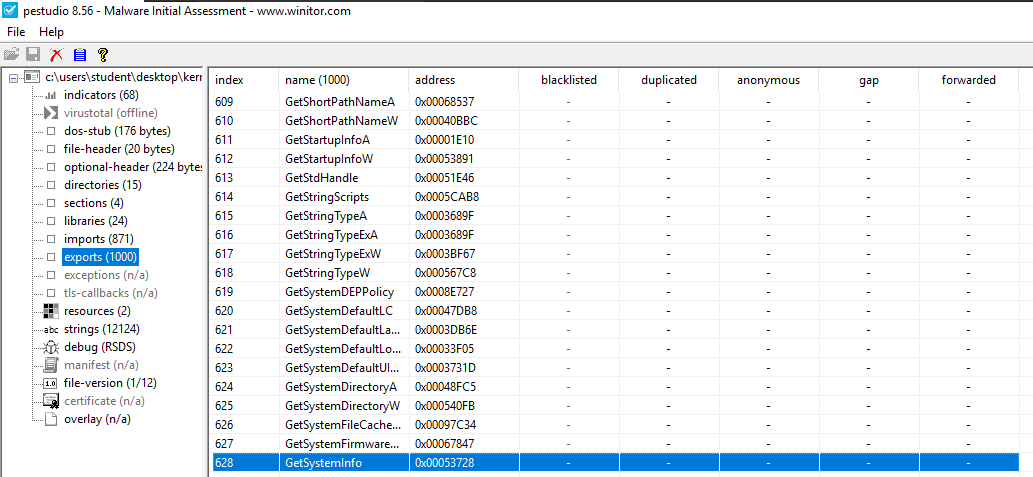
\includegraphics[width=\linewidth]{images/pestudio.png}
\caption{Finding offset of functions using pestudio}
\label{fig:pestudio}
\end{figure}


Subsequently the base address of the libraries loaded in the system must be found. In order to do this the pypanda helper function \lstinline{panda.get_mappings(cpu)} was used. Such function is based on the osi plugin and will return as output a dictionary containing the libraries loaded in the system in that precise moment. This implies that the function will return the libraries loaded by the executable running at the time it was called. By combining it with the syscalls2 plugin it is therefore possible to find out when a specific program is starting to load libraries in the system. In particular the following approach was used: leveraging syscalls2 PPP a callback was placed on the execution of \lstinline{NtMapViewOfSection}. This system call is used by a process to map a file into its memory address space, which is the case of loading libraries from disk. The function designed to execute when the syscall takes place can be seen in Figure \ref{fig:ntmap}. In there if the process running matches the target one the loaded libraries will be extracted and compared against the one containing the api function to be hooked. Once a match is found the function will in turn enable a memory callback \lstinline{cb1} of type \lstinline{PANDA_CB_VIRT_MEM_BEFORE_READ} and then disable itself.

\begin{figure}[htp]
\centering
\begin{lstlisting}[language=Python] 
@panda.ppp("syscalls2", "on_NtMapViewOfSection_return", name="ntmap")
def ntmap(cpu, pc, SectionHandle,  ProcessHandle, BaseAddress, ZeroBits, CommitSize, SectionOffset, ViewSize, InheritDisposition, AllocationType, Win32Protect):
    proc = panda.get_process_name(cpu)
    print(proc)
    if proc == process_name:
        mappings = panda.get_mappings(cpu)
        for mapping in mappings:
            print(
                "Name: "+ffi.string(mapping.name).decode(),
                "Base: 0x{:x} Size: 0x{:x}".format(mapping.base,mapping.size)
            )
            if ffi.string(mapping.name).decode().lower() == "kernel32.dll":
                global base
                base = mapping.base
                global si
                si = mapping.size
                print("Enabling memory callback")
                panda.enable_callback("cb1")
                print("Disabling MapViewOfSections hook")
                panda.disable_ppp("ntmap")
\end{lstlisting}
\caption{\lstinline{NtMapViewOfSection} hooking}
\label{fig:ntmap}
\end{figure}

The memory callback can be seen in Figure \ref{fig:cb1}. It is necessary as when the \lstinline{NtMapViewOfSection} function is called the library is not yet loaded into the reserved virtual memory and therefore placing an hook at an address in that range will not work as it will be overwritten when the content of the dll is loaded. Instead, by monitoring the reserved portion of memory for a read operation, we will be sure that when the read takes place the code will have been loaded in memory and therefore the hook can be place safely. 

\begin{figure}[htp]
\centering
\begin{lstlisting}[language=Python] 
@panda.cb_virt_mem_before_read(name="cb1", procname=process_name, enabled=False)
def virt_mem_after_read(cpu, pc, addr, size):
    if (addr > base and addr < base+si) and base !=0 and si !=0:
        panda.update_hook("sysinfohook",base+0x53728) # offset of GetSystemInfo
        panda.enable_hook("sysinfohook")
        panda.disable_callback("cb1")
        
\end{lstlisting}
\caption{memory callback cb1}
\label{fig:cb1}
\end{figure}

The\lstinline{GetSystemInfo} function is actually really straight forward as it takes in input a pointer to a \lstinline{SYSTEM_INFO} structure that will hold the results, the fields of the structure can be seen in Figure \ref{fig:sysinfo}.

\begin{figure}[htp]
\centering
\begin{lstlisting}[language=C++] 
typedef struct _SYSTEM_INFO {
  union {
    DWORD dwOemId;
    struct {
      WORD wProcessorArchitecture;
      WORD wReserved;
    } DUMMYSTRUCTNAME;
  } DUMMYUNIONNAME;
  DWORD     dwPageSize;
  LPVOID    lpMinimumApplicationAddress;
  LPVOID    lpMaximumApplicationAddress;
  DWORD_PTR dwActiveProcessorMask;
  DWORD     dwNumberOfProcessors;
  DWORD     dwProcessorType;
  DWORD     dwAllocationGranularity;
  WORD      wProcessorLevel;
  WORD      wProcessorRevision;
} SYSTEM_INFO, *LPSYSTEM_INFO;
\end{lstlisting}
\caption{\lstinline{STYSTEM_INFO} structure.}
\label{fig:sysinfo}
\end{figure}

The content of this structure will be populated after the function executes therefore in order to correctly modify the \lstinline{dwNumberOfProcessors} field, which is the one checked by ParanoidFish, it is necessary to obtain the return address at which the function will jump after the execution. In this way the structure will have already been populated and the fields can be safely modified.

This can be achieved by saving the return address placed on the stack when the function is called and setting a breakpoint on such address. In this way the address of the structure can be extracted from the stack once the function returns and then the \lstinline{dwNumberOfProcessors} field patched.  


As mentioned before the use of Python provides great flexibility not only in plugin writing but also on the automation side. In order to automate the analysis the record and replay actions have been automated inside the python script. To achieve this the hooks2 plugin was used, such plugin is designed to substitute the hooks one. Although it is not yet finished it already provides some useful callbacks, in particular the \lstinline{on_process_start} and \lstinline{on_process_end} callbacks have been used to start and stop the recording. Some checks have been put in place in order to execute the code only if the process is the one monitored and only if the script is being run on a live system. Details of such functions can be seen in \ref{fig:startstop}

\begin{figure}[htp]
\centering
\begin{lstlisting}[language=Python] 
# Only used to take recordings of patched sessions
@panda.ppp("hooks2", "on_process_start")
def rec(cpu, procname, asid, pid):
    print(ffi.string(procname).decode())
    if ffi.string(procname).decode() == process_name:
        print(ffi.string(procname).decode()," Started!")
        if not rep:
            panda.run_monitor_cmd("begin_record rec")

@panda.ppp("hooks2", "on_process_end")
def end_rec(cpu, procname, asid, pid):
    if (ffi.string(procname).decode() == process_name) and not rep:
        panda.disable_callback("hyper")
        panda.disable_hook("sysinfohook")
        panda.disable_hook("patchsysinfo")
        panda.disable_ppp("ntmap")
        panda.run_monitor_cmd("end_record")
\end{lstlisting}
\caption{functions used to start and stop the recording.}
\label{fig:startstop}
\end{figure}


\subsection{Faking time results}

Another important fingerprinting technique consists in checking the Time Stamp Counter (TSC) of the system in order to check the time elapsed between different instructions. Most CPUs provide a dedicated instruction to access the TSC called RDTSC, the most common fingerprinting techniques involve checking the time elapsed between two subsequent execution of RDTSC or fingerprinting the time it takes for a VM Exit to happen. A simple VM exit can be generated with CPUID as it is a privileged instruction as explained in Chaper \ref{chap:2}.

One of the limitation of \textbf{PANDA} is that it does not provide a callback able to intercept all the types of hypervisor call such as CPUID and RDTSC but, instead, CPUID is the only one associated with \lstinline{PANDA_CB_GUEST_HYPERCALL}. Therefore, in order to manipulated the TSC of the emulated system, it was necessary to introduce some modifications inside the \textbf{PANDA} code base an in particular to add a new callback specifically dedicated to the RDTSC instruction. 

\textbf{PANDA} already provides the possibility to create Plugin to Plugin interfaces which are particular types of callbacks. However, those can only be based on functions already exposed by the \textbf{PANDA} api which does not provide the necessary level of control over the emulated architecture. Instead a new "native" callback was created for TSC handling named \lstinline{PANDA_CB_RDTSC}. 

In order to do this it is first necessary to understand how QEMU handles the TSC counter for the guest Operating System and how \textbf{PANDA} callbacks works internally. On this last point it was not possible to find any reference about extending \textbf{PANDA} functionalities inside the documentation and therefore the source code had to be manually interpreted in order to find out where the modifications should take place.

The files involved in the creation of "native" callbacks are the following: 

\begin{itemize}
    \item \lstinline{./panda/include/panda/callbacks/cb-defs.h} this header file holds the declaration of the \lstinline{panda_cb_type} type as well as a union of all possible callback function types.
    
    The modifications introduced in this file in order to support a new callback can be seen in Figure \ref{fig:mod1}.
    
    \begin{figure}[htp]
    \centering
    \begin{lstlisting}[language=C]
    typedef enum panda_cb_type {
        [...]
        PANDA_CB_RDTSC, // <- New callback
        PANDA_CB_LAST
    } panda_cb_type;
    
    // Union of all possible callback function types
    typedef union panda_cb {
        [...]
        bool (*rdtsc)(CPUState *env, uint64_t val); // <- New callback
    } panda_cb;
    \end{lstlisting}
    \caption{\textbf{cb-defs.h} modifications}
    \label{fig:mod1}
    \end{figure}
        
    \item \lstinline{./panda/include/panda/callbacks/cb-support.h} this header file contains the signatures for the \textbf{PANDA} callback helper functions. The helpers essentially iterate over the list of registered callbacks and invoke them with the appropriate arguments. In this file was added the signature of the new callback helper function: 
    \lstinline{bool panda_callbacks_rdtsc(CPUState *env, uint64_t val);}
    
    \item \lstinline{./panda/src/cb-support.c} this file contains the description of how the callback should be build. In particular teh \lstinline{cb-macros.h} file defines some custom functions: \lstinline{MAKE_CALLBACK} and \lstinline{MAKE_REPLAY_ONLY_CALLBACK} that will take care of generating the callback helper function. The following line was added to this file: \lstinline{MAKE_CALLBACK(bool, RDTSC, rdtsc, CPUState*, env, uint64_t, val);}
    
\end{itemize}

Once the callback has been defined in the above mentioned \textbf{PANDA} files it can be used inside the code. In particular in order for a callback to work it must specified at which point of the emulation the callback should be invoked. For example the \lstinline{PANDA_CB_BEFORE_BLOCK_EXEC}, which is called before a basic block is executed(Figure \ref{fig:calls}), is implemented with the \lstinline{panda_callbacks_before_block_exec(CPUState *env, TranslationBlock *tb);} which is then called in the \lstinline{cpu_tb_exec} function inside the main emulator file (\lstinline{./cpu-exec.c}).

In the case of RDTSC it was first necessary to track down how QEMU manages such counter in the virtual CPU. There are 3 different places in which the TSC counter is managed:

\begin{itemize}
    \item The \lstinline{cpu_get_ticks} function returns the time elapsed inside the VM. This function is implemented in \lstinline{./cpus.c} and is directly connected to the host one as it calls the \lstinline{cpu_get_host_ticks}.
    \item The above function is then called in the \lstinline{cpu_get_tsc} which is the function called in the i386 cpu implementation to handle the tsc counter. 
    \item Lastly in the \lstinline{./target/i386/misc_helper.c} there is a function called \lstinline{helper_rdtsc} which takes care of handling the RDTSC instruction inside the guest. This appears to be the best place in which to place the callback function. As a matter of fact this is the same file in which the CPUID hooking function is placed. 
\end{itemize}

The logic to implement this callback is partially inspired to the one used in the \lstinline{PANDA_CB_GUEST_HYPERCALL}. The \lstinline{panda_callbacks_rdtsc} function is called inside \lstinline{helper_rdtsc}, the return type of the callback is boolean meaning that the plugin using it can signal if RDTSC has been handled or not. In particular, if the callback returns \textit{true}, the values of TSC are not copied in the RAX and RDX registers but it is assumed that the plugin has taken care of populating the registers with the correct value. On the other hand, if the callback returns \textit{false}, the normal execution continues and the registers are populated with the correct values. 

The TSC value is also passed to \lstinline{panda_callbacks_rdtsc} under the \lstinline{val} parameter. In this way the plugin has a direct and convenient access to the Timestamp that would have been used to populate the registers and can manipulate it accordingly.

The function responsible to patch RDTSC in the plugin can be seen in Figure \ref{fig:rdtscpatch}. The approach taken here was to bring down TSC difference by dividing the value by an arbitrary number. Such number was calculated empirically and depends is dependant on the system running and on the number of plugins loaded as the execution time will vary based on the load of the emulated system.

\begin{figure}[htp]
\centering
\begin{lstlisting}[language=C]
bool rdtsc(CPUState *cpu, uint64_t val){
    if (rdtsc_patch==1){
        if (check_pid(cpu,tname)){ // we need this here otherwise it will segfault
            val=val/10000;
            EAX = (uint32_t)(val);
            EDX = (uint32_t)(val >> 32);
            printf("[DEBUG] rdtsc patched!\n");
            return true;
        }
    }
    return false;
}
\end{lstlisting}
\caption{\textbf{cb-defs.h} modifications}
\label{fig:rdtscpatch}
\end{figure}

This plugin can also be combined with CPUID in order to specifically patch RDTSC if it is called to fingerprint the time taken by a VM Exit to be handled. 

In order to test if this plugin was working and also test the performances of the fully emulated system it was necessary to write a custom test program. This can be found in Figure \ref{fig:rdttest}. The goal was to check the difference in time between two different calls of RDTSC in order to:

\begin{enumerate}
    \item Define a baseline of the time taken by instructions to be executed on a bare metal system Figure \ref{fig:bmetal}.
    \item Determine the time it takes to execute the same instruction under full system emulation Figure \ref{fig:rdtsc1}(a). This is particularly challenging as the more plugins are used in the system the more it takes for the entire emulation to run. The results in the Figure \ref{fig:rdtsc1}(a) were obtained with all the above created plugins loaded. 
\end{enumerate}


\begin{figure}[htp]
\centering
\begin{lstlisting}[language=C]
#include <windows.h>
#include <stdio.h>

void test1(){
    unsigned long long ret, ret1, ret2;
	unsigned eax, edx;
    for (int i=0;i<11;i++){
        __asm__ volatile("rdtsc" : "=a" (eax), "=d" (edx));
        ret  = ((unsigned long long)eax);
        __asm__ volatile("rdtsc" : "=a" (eax), "=d" (edx));
        ret1  = ((unsigned long long)eax);

        printf("First call %llu\n",ret);
        printf("Second call %llu\n",ret1);

        printf("Difference %llu\n",ret1-ret);
    }

    __asm__ volatile("rdtsc" : "=a" (eax), "=d" (edx));
    ret  = ((unsigned long long)eax) | (((unsigned long long)edx) << 32);
	
	__asm__ volatile("cpuid" : /* no output */ : "a"(0x00));
	
	__asm__ volatile("rdtsc" : "=a" (eax), "=d" (edx));
	ret2  = ((unsigned long long)eax) | (((unsigned long long)edx) << 32);
    printf("VM exit %llu\n",ret2-ret);
}



int main(){
    printf("Calling test1\n");
    test1();
    getchar();
    return 0;
}
\end{lstlisting}
\caption{RDTSC testing program}
\label{fig:rdttest}
\end{figure}

\begin{figure}%
    \centering
    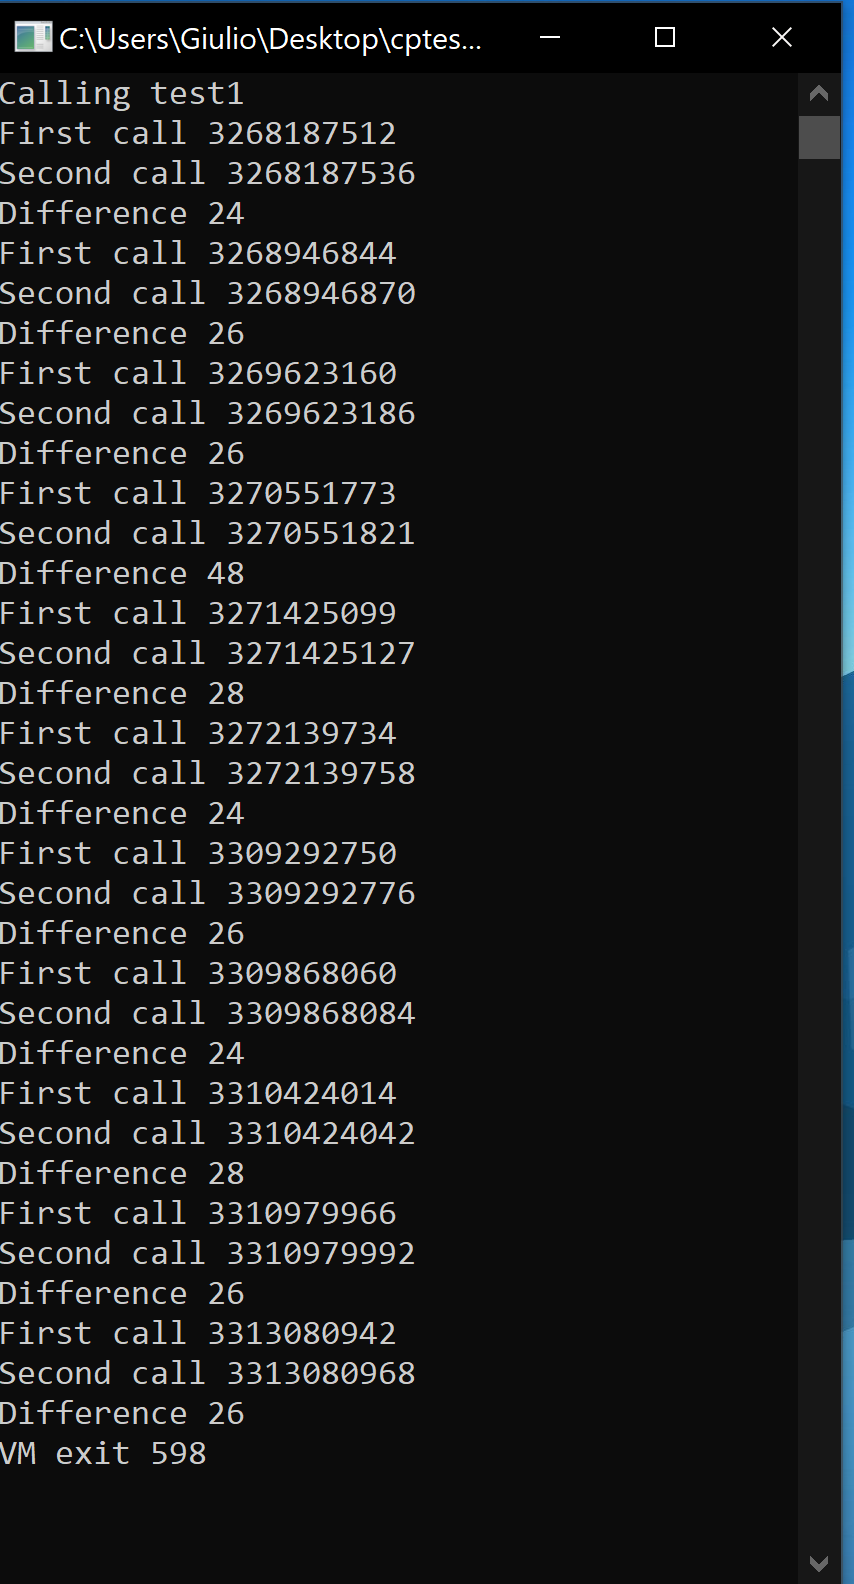
\includegraphics[width=0.6\linewidth]{images/bmetal.PNG}%
    \caption{Results of running RDTSC test program on a bare metal machine}%
    \label{fig:bmetal}%
\end{figure}

\begin{figure}%
    \centering
    \subfloat[\centering vanilla system]{{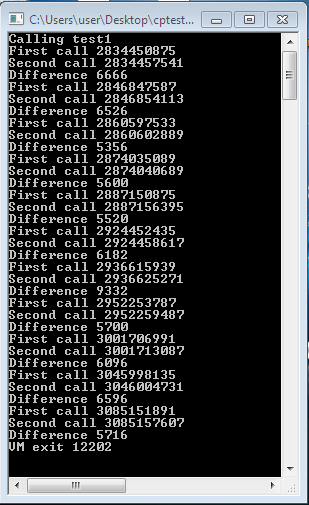
\includegraphics[width=0.5\linewidth]{images/cptest2.png} }}%
    \subfloat[\centering plugin]{{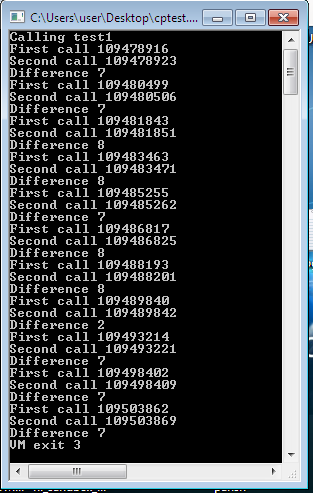
\includegraphics[width=0.5\linewidth]{images/cptest3.png} }}%
    \caption{Results of running RDTSC without the patch (a) and with the \lstinline{timing_patch} plugin applied (b)}%
    \label{fig:rdtsc1}%
\end{figure}

Lastly in Figure\ref{fig:rdtsc1}(b) it is possible to see how the plugin is able to effectively patch the RDTSC instruction faking the result of that instruction by overwriting the values in the EAX and EDX registries. 

\section{Results}

In order to benchmark the newly created plugins it was decided to use the two most common and complete tools: ParanoidFish and Al-Khaser.

In Figure \ref{fig:res} it is possible to see how the execution of Paranoid Fish on a system with all plugins enabled compares to a vanilla execution. 

In Figure \ref{fig:res1} it is possible to see how the execution of Al-Khaser compares to a vanilla execution. 


It is possible to see how some tests are still flagged as failed. For example the disk one can easily be fixed by creating a bigger virtual hard disk. The WMI ones are particularly interesting as it requires a deep understanding of how WMI is treated inside windows and how it can be patched. A detailed discussion on this can be found in the next chapter. 


\chapter{Conclusions and Future Works}

\section{Conclusions}

\section{Future Works}

\backmatter
% bibliography
\cleardoublepage
\phantomsection
\bibliographystyle{unsrt} % BibTeX style
\bibliography{bibliography} % BibTeX database without .bib extension

\end{document}
